\section{Per-Fragment Operations}

\subsection{Overview}
\begin{frame}{Per-Fragment Operations Stage}
  \begin{columns}
    \small
    \begin{column}{0.7\textwidth}
      \begin{raybox}{Per-Fragment Operations}
        \textbf{Input:} Colored fragments from fragment shader \\
        \textbf{Output:} Final pixels to framebuffer

        \vspace{0.3cm}
        \textbf{Fixed-function tests and operations:}
        \begin{itemize}
          \item Scissor test
          \item Stencil test
          \item Depth test
          \item Alpha blending
        \end{itemize}
      \end{raybox}
    \end{column}
    \begin{column}{0.3\textwidth}
      \begin{tikzpicture}[scale=0.7]
        % Input fragments
        \foreach \i in {0,1,2} {
          \foreach \j in {0,1,2} {
            \fill[AccentColor!30] (\i*0.4, \j*0.4 + 3) circle (0.1);
          }
        }
        \node[below] at (0.4, 2.5) {\scriptsize Coloured Fragments};

        % Fragment shader box

        \node[rectangle, draw, fill=PrimaryColor!30, minimum width=1.5cm, minimum height=1cm] (fs) at (0.4,0.5) {
          \begin{minipage}{2cm}
            \centering
            \textbf{Per Fragment} \\
            \textbf{Ops}
          \end{minipage}
        };

        % Output colored fragments
        \begin{scope}[yshift=-2cm]
          \foreach \i in {0,1,2} {
            \foreach \j in {0,1,2} {
              \fill[ObjectColor] (\i*0.4, \j*0.4) circle (0.1);
            }
          }
          \node[below] at (0.4, -0.3) {\scriptsize Final};
          \node[below] at (0.4, -0.7) {\scriptsize Fragments};
        \end{scope}

        % Arrows
        \draw[->, thick, AccentColor] (0.4,1.8) -- (0.4,1.2);
        \draw[->, thick, AccentColor] (0.4,-0.2) -- (0.4,-0.8);
      \end{tikzpicture}
    \end{column}
  \end{columns}
\end{frame}

\subsection{Pipeline Flow}
\begin{frame}{Per-Fragment Operations Pipeline}
  \small
  \begin{conceptbox}{Fixed-Function Stage}
    \textbf{Non-programmable} stage with configurable tests and operations

    \vspace{0.3cm}
    \textbf{Sequential processing:} Each fragment goes through all enabled tests
  \end{conceptbox}

  \vspace{0.3cm}
  \begin{center}
    \begin{tikzpicture}[scale=0.8, every node/.style={font=\footnotesize}]
      % Fragment input
      \node[rectangle, draw, fill=AccentColor!30, minimum width=1.5cm, minimum height=0.6cm] (frag) at (0,4) {Fragment};

      % Tests
      \node[rectangle, draw, fill=LightGray!50, minimum width=1.5cm, minimum height=0.6cm] (scissor) at (0,3) {Scissor Test};
      \node[rectangle, draw, fill=LightGray!50, minimum width=1.5cm, minimum height=0.6cm] (stencil) at (0,2) {Stencil Test};
      \node[rectangle, draw, fill=LightGray!50, minimum width=1.5cm, minimum height=0.6cm] (depth) at (0,1) {Depth Test};
      \node[rectangle, draw, fill=LightGray!50, minimum width=1.5cm, minimum height=0.6cm] (blend) at (0,0) {Blending};

      % Success path
      \foreach \i/\j in {frag/scissor, scissor/stencil, stencil/depth, depth/blend} {
        \draw[->, thick, green!70!black] (\i) -- (\j);
      }

      % Discard paths
      \node[right] at (1.5,3) {\color{red} \scriptsize Discard if outside scissor};
      \node[right] at (1.5,2) {\color{red} \scriptsize Discard if stencil test fails};
      \node[right] at (1.5,1) {\color{red} \scriptsize Discard if depth test fails};
      \node[right] at (1.5,0) {\scriptsize Blends based on alpha value};

      % Final output
      \node[rectangle, draw, fill=ObjectColor!30, minimum width=1.5cm, minimum height=0.6cm] (fb) at (0,-1) {Framebuffer};
      \draw[->, thick, green!70!black] (blend) -- (fb);
    \end{tikzpicture}
  \end{center}
\end{frame}

\subsection{Depth Testing}
\begin{frame}{Depth Testing}
  \footnotesize
  \begin{columns}
    \begin{column}{0.7\textwidth}
      \begin{raybox}{Z-Buffer Algorithm}
        \textbf{Purpose:} Determine which fragments are visible

        \vspace{0.3cm}
        \textbf{Process:}
        \begin{enumerate}
          \item Compare fragment depth with stored depth
          \item If test passes, update color and depth buffers
          \item If test fails, discard fragment
        \end{enumerate}

        \vspace{0.3cm}
        \textbf{Common depth functions:}
        \begin{itemize}
          \item \texttt{GL\_LESS} - Default, closer objects win
          \item \texttt{GL\_LEQUAL} - Less than or equal
          \item \texttt{GL\_GREATER} - Farther objects win
          \item \texttt{GL\_ALWAYS} - Always pass (no depth testing)
        \end{itemize}
      \end{raybox}
    \end{column}
    \begin{column}{0.3\textwidth}
      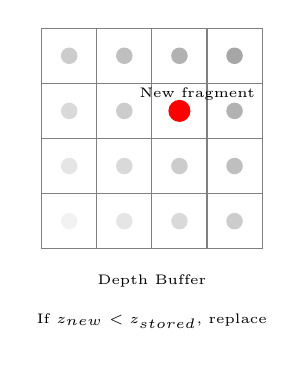
\begin{tikzpicture}[scale=0.7]
        % Z-buffer visualization
        \draw[gray] (0,0) grid (4,4);
        \node[below] at (2,-0.3) {\tiny Depth Buffer};

        % Different depth values
        \foreach \i in {0,1,2,3} {
          \foreach \j in {0,1,2,3} {
            \pgfmathparse{(\i+\j)*10+10}
            \fill[gray!\pgfmathresult] (\i+0.5,\j+0.5) circle (0.15);
          }
        }

        % New fragment
        \fill[red] (2.5,2.5) circle (0.2);
        \node[right] at (1.6,2.8) {\tiny New fragment};

        % Depth comparison
        \node[below] at (2,-1) {\tiny If $z_{new} < z_{stored}$, replace};
      \end{tikzpicture}
    \end{column}
  \end{columns}
\end{frame}

\begin{frame}{Early Z-Testing Optimization}
  \footnotesize
  \begin{columns}
    \begin{column}{0.6\textwidth}
      \begin{conceptbox}{Early Depth Test}
        \textbf{Optimization:} Perform depth test \emph{before} fragment shader

        \vspace{0.3cm}
        \textbf{Benefits:}
        \begin{itemize}
          \item Avoid expensive fragment shader execution
          \item Significant performance improvement
          \item Especially effective for complex shaders
        \end{itemize}

        \vspace{0.3cm}
        \textbf{Limitations:}
        \begin{itemize}
          \item Fragment shader cannot modify depth
          \item No alpha testing in fragment shader
          \item Must be enabled/supported by hardware
        \end{itemize}
      \end{conceptbox}
    \end{column}
    \begin{column}{0.4\textwidth}
      \begin{tikzpicture}[scale=0.5]
        % Traditional pipeline
        \begin{scope}[yshift=2cm]
          \node[rectangle, draw, fill=AccentColor!30, minimum width=1.2cm, minimum height=0.5cm] (rast1) at (0,0) {\tiny Raster};
          \node[rectangle, draw, fill=PrimaryColor!30, minimum width=1.2cm, minimum height=0.5cm] (fs1) at (3,0) {\tiny Frag Shader};
          \node[rectangle, draw, fill=LightGray, minimum width=1.2cm, minimum height=0.5cm] (depth1) at (6,0) {\tiny Depth Test};

          \draw[->, thick] (rast1) -- (fs1);
          \draw[->, thick] (fs1) -- (depth1);
          \node[above] at (3,0.8) {\tiny Traditional};
        \end{scope}

        % Early Z pipeline
        \begin{scope}[yshift=0cm]
          \node[rectangle, draw, fill=AccentColor!30, minimum width=1.2cm, minimum height=0.5cm] (rast2) at (0,0) {\tiny Raster};
          \node[rectangle, draw, fill=LightGray, minimum width=1.2cm, minimum height=0.5cm] (depth2) at (3,0) {\tiny Early Z};
          \node[rectangle, draw, fill=PrimaryColor!30, minimum width=1.2cm, minimum height=0.5cm] (fs2) at (6,0) {\tiny Frag Shader};

          \draw[->, thick] (rast2) -- (depth2);
          \draw[->, thick] (depth2) -- (fs2);
          \draw[->, thick, red] (depth2) -- (2,-1) node[below] {\tiny Discard};
          \node[above] at (3,0.6) {\tiny Early Z};
        \end{scope}
      \end{tikzpicture}
    \end{column}
  \end{columns}
\end{frame}

\subsection{Alpha Blending}
\begin{frame}{Alpha Blending}
  \footnotesize
  \begin{columns}
    \begin{column}{0.55\textwidth}
      \begin{raybox}{Transparency via Blending}
        \textbf{Purpose:} Combine fragment color with framebuffer color

        \vspace{0.3cm}
        \textbf{Standard alpha blending:}
        \begin{align*}
          C_{result} &= C_{src} \cdot \textcolor{red}{\alpha_{src}} + C_{dst} \cdot \textcolor{blue}{ (1 - \alpha_{src})}
        \end{align*}

        \vspace{0.3cm}
        \textbf{Blend equation components:}
        \begin{itemize}
          \item $C_{src}$ = source color (fragment)
          \item $C_{dst}$ = destination color (framebuffer)
          \item $\alpha_{src}$ = source alpha value
        \end{itemize}
      \end{raybox}
    \end{column}
    \begin{column}{0.45\textwidth}
      \begin{center}
        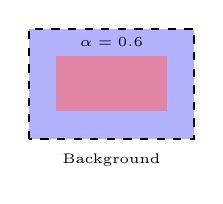
\begin{tikzpicture}[scale=0.7]
          % Background
          \fill[blue!30] (0,0) rectangle (3,2);
          \node[below] at (1.5,-0.1) {\tiny Background};

          % Transparent overlay
          \fill[red!60, opacity=0.6] (0.5,0.5) rectangle (2.5,1.5);
          \node[above] at (1.5,1.5) {\tiny $\alpha = 0.6$};

          % Result
          \draw[thick, dashed] (0,0) rectangle (3,2);
        \end{tikzpicture}
      \end{center}

      \begin{mathbox}{Blend Functions}
        \scriptsize
        \textbf{Common source factors:}
        \begin{itemize}
          \item \texttt{GL\_SRC\_ALPHA}
          \item \texttt{GL\_ONE}
          \item \texttt{GL\_ZERO}
        \end{itemize}

        \textbf{Common dest factors:}
        \begin{itemize}
          \item \texttt{GL\_ONE\_MINUS\_SRC\_ALPHA}
          \item \texttt{GL\_ONE}
          \item \texttt{GL\_DST\_ALPHA}
        \end{itemize}
      \end{mathbox}
    \end{column}
  \end{columns}
\end{frame}

\begin{frame}{Advanced Blending Modes}
  \footnotesize
  \begin{columns}
    \begin{column}{0.5\textwidth}
      \begin{conceptbox}{Additive Blending}
        \textbf{Formula:} $C_{result} = C_{src} + C_{dst}$

        \textbf{Use cases:}
        \begin{itemize}
          \item Fire, explosions, energy effects
          \item Light accumulation
          \item Particle systems
        \end{itemize}
      \end{conceptbox}

      \begin{conceptbox}{Multiplicative Blending}
        \textbf{Formula:} $C_{result} = C_{src} \times C_{dst}$

        \textbf{Use cases:}
        \begin{itemize}
          \item Shadows, darkening effects
          \item Color filtering
          \item Atmospheric effects
        \end{itemize}
      \end{conceptbox}
    \end{column}
    \begin{column}{0.5\textwidth}
      \begin{conceptbox}{Screen Blending}
        \textbf{Formula:} $C_{result} = 1 - (1 - C_{src})(1 - C_{dst})$

        \textbf{Use cases:}
        \begin{itemize}
          \item Brightening effects
          \item Light overlays
          \item Highlight enhancement
        \end{itemize}
      \end{conceptbox}

      \begin{raybox}{Order Dependency}
        \textbf{Problem:} Blending is order-dependent

        \textbf{Solutions:}
        \begin{itemize}
          \item Sort transparent objects back-to-front
          \item Order-independent transparency (OIT)
        \end{itemize}
      \end{raybox}
    \end{column}
  \end{columns}
\end{frame}

\subsection{Additional Operations}
\begin{frame}{Additional Per-Fragment Operations}
  \scriptsize
  \begin{columns}
    \begin{column}{0.5\textwidth}
      \begin{raybox}{Stencil Test}
        \textbf{Purpose:} Per-pixel masking and control flow

        \textbf{How it works:}
        \begin{itemize}
          \item Each pixel stores an 8-bit stencil value
          \item Compare fragment’s stencil to buffer value
          \item Conditionally discard fragment based on test
          \item Can also update stencil buffer (e.g., increment)
        \end{itemize}

        \textbf{Applications:}
        \begin{itemize}
          \item Object outlining
          \item Mirror/portal rendering
          \item Shadow volumes
          \item UI masking
        \end{itemize}
      \end{raybox}
    \end{column}

    \begin{column}{0.5\textwidth}
      \begin{conceptbox}{Scissor Test}
        \textbf{Purpose:} Rectangular clipping region

        \vspace{0.2cm}
        \textbf{Use cases:}
        \begin{itemize}
          \item Discard fragments outside defined rectangle
          \item UI rendering, viewport masking
          \item Very efficient and hardware-accelerated
        \end{itemize}
      \end{conceptbox}

      \begin{conceptbox}{Others}
        \textbf{Less common operations:}
        \begin{itemize}
          \item \textbf{Dithering:} Adds noise to smooth color gradients
          \item \textbf{Logic Ops:} Bitwise operations on output color
          \item \textbf{Occlusion Queries:} Count visible fragments
        \end{itemize}
      \end{conceptbox}
    \end{column}
  \end{columns}
\end{frame}
